% ===========================
%       Chapter 1A.5
%         Proteins
%   Created by Michael Tang
%        2025.01.01
% ===========================

\subsubsection{1A.5 \underline{Proteins} (蛋白质)}
\paragraph{Introduction to Proteins} Proteins are macromolecules essential to numerous biological processes. They are composed of
long chains of amino acids linked by \underline{peptide bonds} (肽键). Functions of proteins include:
\begin{itemize}
    \item Providing structural support (e.g., hair, skin, and nails).
    \item Acting as \underline{enzymes} (酶) for \underline{metabolism} (新陈代谢) and \underline{digestion} (消化).
    \item Regulating \underline{hormones} (激素).
    \item Transporting oxygen (e.g., hemoglobin 血红蛋白).
    \item Supporting \underline{immune defense} (免疫防御).
\end{itemize}
Proteins are made of carbon, hydrogen, oxygen, and nitrogen, with some containing sulfur. They are synthesized by linking amino
acids through condensation reactions. There are about 20 different naturally occurring amino acids that can combine in different
ways to produce a wide range of different proteins.

\paragraph{Amino Acids: The Building Blocks of Proteins}
All amino acids share the same basic structure:
\begin{itemize}
    \item An amino group (\ce{-NH2} 氨基).
    \item A \underline{carboxyl group} (\ce{-COOH} 羧基).
    \item A variable $R$ group (side chain) unique to each amino acid.
\end{itemize}
The $R$ group determines the properties and function of the amino acid, influencing whether it is \underline{hydrophobic} (疏水的),
\underline{hydrophilic} (亲水的), or changed.
\begin{figure}[H]
    \centering
    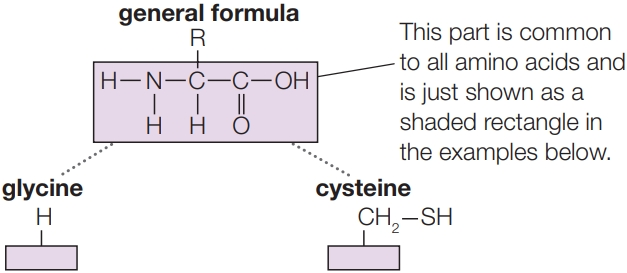
\includegraphics[scale=0.35]{Biology/1A/Images/1A-5-1.png}
    \caption{Some different amino acids. In the simplest amino acid, \underline{glycine} (甘氨酸), $R$ is a single hydrogen atom.
    In a larger amino acid such as \underline{cysteine} (半胱氨酸), $R$ is much more complex.}
\end{figure}

\paragraph{Formation of Proteins}
Proteins are formed by condensation reactions:
\begin{itemize}
    \item \textbf{Peptide bonds} form between the carboxyl group of one amino acid and the amino group of another, releasing a
    molecule of water.
    \begin{figure}[H]
        \centering
        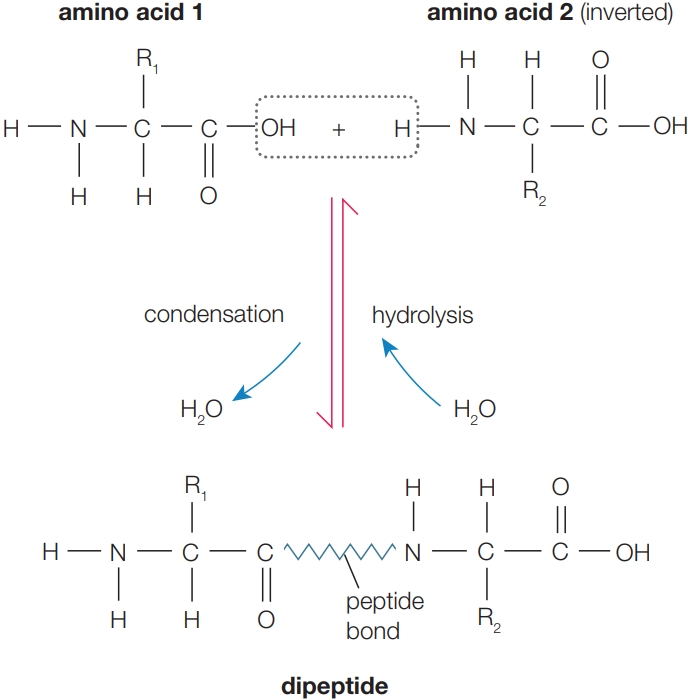
\includegraphics[scale=0.35]{Biology/1A/Images/1A-5-2.png}
        \caption{Amino acids are the building blocks of proteins, joined together by peptide bonds.}
    \end{figure}
    \item Chains of amino acids linked by peptide bonds are called \underline{polypeptides} (多肽). These fold to create
    functional proteins. The peptide bond between amino acids is a strong bond. Other bonds are also made between amino acids in
    a chain, to create the 3D structure of the protein. They depend on the atoms in the $R$ group and include hydrogen bonds,
    \underline{disulfide bridges} (二硫键), and ionic bonds.
    \begin{figure}[H]
        \centering
        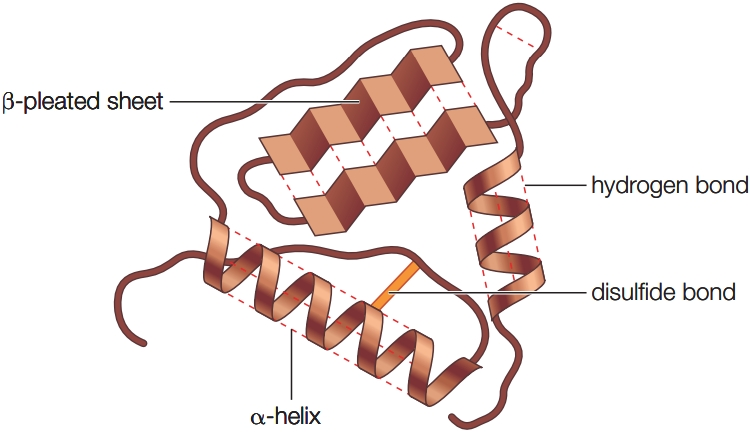
\includegraphics[scale=0.3]{Biology/1A/Images/1A-5-3.png}
        \caption{Hydrogen bonds and disulfide bonds maintain the shape of protein molecules and this determines their function.}
    \end{figure}
\end{itemize}

\paragraph{Protein Structure Levels} Proteins \underline{exhibit} (表现) four levels of structure:
\begin{figure}[H]
    \centering
    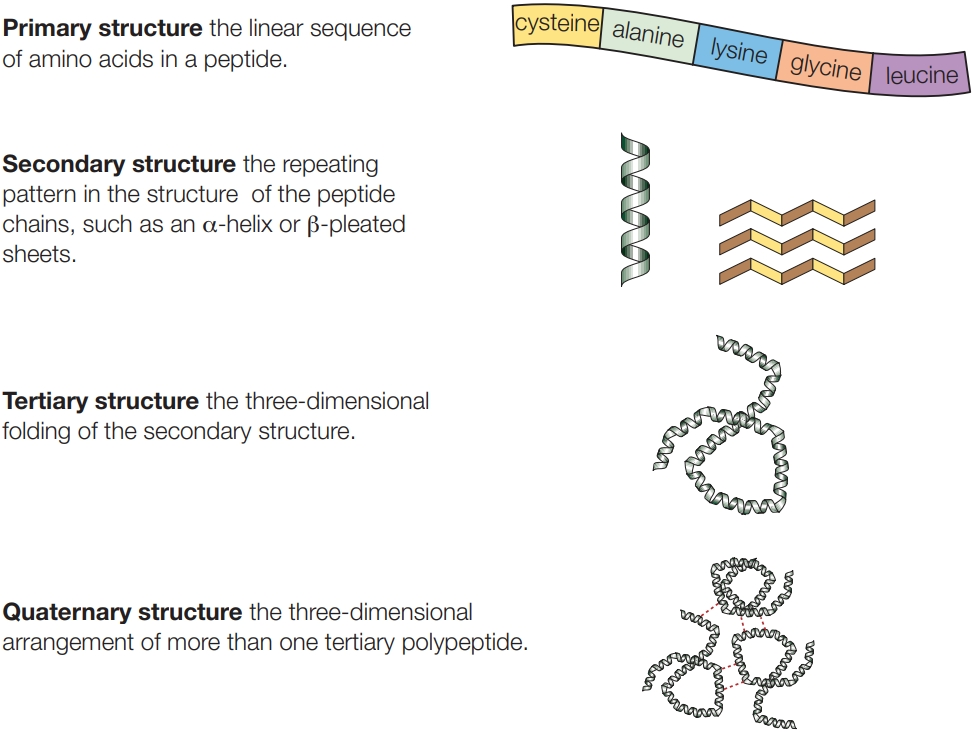
\includegraphics[scale=0.4]{Biology/1A/Images/1A-5-4.png}
    \caption{The 3D structure of proteins.}
\end{figure}

\paragraph{Types of Proteins}
\begin{itemize}
    \item[1.] \textbf{Fibrous Proteins} (纤维蛋白质) are long, insoluble proteins that provide structural support. Examples include
    \underline{collagen} (胶原蛋白) in skin and \underline{keratin} (角蛋白) in hair.
    \begin{figure}[H]
        \centering
        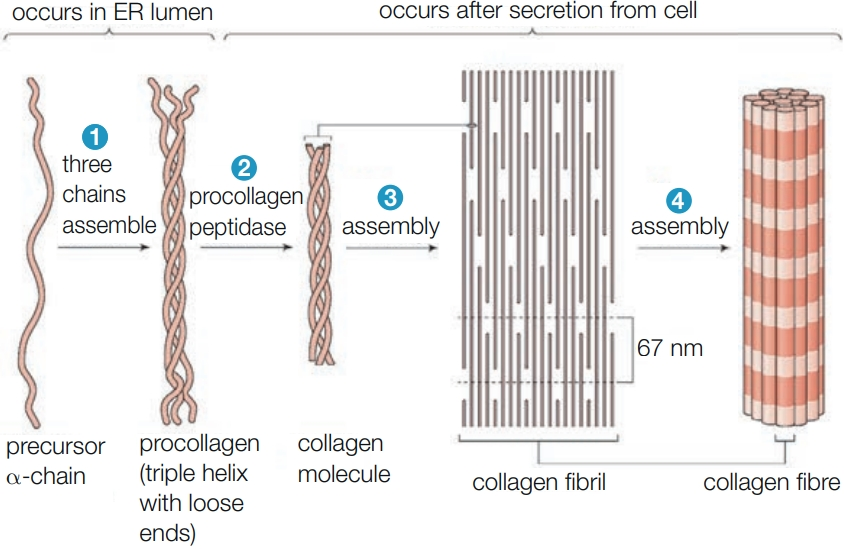
\includegraphics[scale=0.3]{Biology/1A/Images/1A-5-5.png}
        \caption{Collagen is a fibrous protein with an unusual triple helix structure and immense strength.}
    \end{figure}
    \item[2.] \textbf{Globular Proteins} (球蛋白质) are compact, spherical proteins with metabolic functions. Examples include
    \underline{enzymes} and \underline{hemoglobin}.
\end{itemize}

\paragraph{\underline{Denaturation} (变性) of Proteins}
When proteins are exposed to extreme pH or temperature changes, they lose their 3D structure and functionality. This process is
called denaturation.

\paragraph{Testing for Proteins}
\underline{Biuret Test} (比约特试验) is used to test for the presence of proteins:
\begin{itemize}
    \item Add Biuret reagent (sodium hydroxide and copper sulfate).
    \item A purple color indicates the presence of proteins.
\end{itemize}